\documentclass[fontsize=12pt]{scrartcl}
\usepackage[ngerman]{babel}
\usepackage[utf8]{inputenc}
%\usepackage[latin1]{inputenc}
\usepackage{amsmath}
\usepackage{amstext}
\usepackage{amssymb}
\usepackage{stmaryrd}
\usepackage{verbatim}
\usepackage{mathrsfs}
\usepackage{extarrows}
\usepackage[arrow, matrix, curve]{xy}
\usepackage[centering,includeheadfoot,margin=2cm]{geometry}
\usepackage{gensymb}
\usepackage{graphicx}
\usepackage{framed}
\usepackage{xcolor}
\usepackage{float}
\usepackage{graphicx} 
\usepackage{sidecap}
\usepackage{blindtext,wrapfig}
\usepackage{epstopdf}
\usepackage{import}
\usepackage{fancyhdr}
\usepackage{fancybox}
\usepackage{graphicx}
\usepackage{caption}
\usepackage{subcaption}
\DeclareGraphicsRule{.tif}{png}{.png}{`convert #1 `basename #1 .tif`.png} 
\pagestyle{fancy}
\fancyhf{}
\fancyhead[R]{Physiklaisches Praktikum 1}
\fancyhead[L]{Linda Werneck, Gentian Rrafshi}
\fancyfoot[R]{Seite \thepage}
\fancyfoot[L]{\today}

\begin{document}

\begin{minipage}{\textwidth}
\begin{center}\large
\title{S12b – Ultraschallwellen nach Debye-Sears \\
		~\\
		~\\
		Assistent: Michael Schmid \\
		Datum Versuchsdurchführung: \\
		15.04.2015}

\author{bearbeitet von\\
		Gruppe 3-031: \\
		Linda Werneck Matrnr. 2901495 \\
		Gentian Rrafshi Matrnr. 2721617 }
\date{\today}

\maketitle

\end{center}
\end{minipage}

\newpage

\tableofcontents

\newpage
\noindent

\section{ Versuchsziel}

Ziel des Versuchs ist die Ermittlung der Schallgeschwindigkeit und der Schallwellenlänge in destilliertem Wasser und in einem Glycerin-Wasser-Gemisch mithilfe von Lichtbeugung nach dem Debye-Sears- Effekt. Zudem soll das Kompressionsmodul errechnet werden.\\
\textbf{Anmerkung:}\\
Da die Geräte bei der Gruppe 3-043 nicht funktionierten, ist diese Gruppe nach Anordnung vom Assistenten zu uns hinzugestoßen. Wir haben uns darauf geeinigt, dass wir, Linda Werneck, Gentian Rrafshi den ersten Versuchsdurchgang machen und die andere Gruppe den zweiten Durchgang macht.

\section{ Grundlagen}

In diesem Versuch geht es um Schallwellen, welche akustische und elastische Longitudinalwellen sind, d.h. Wellen sind, die in Ausbreitungsrichtung schwingen. Wie alle physikalischen Wellen genügt die Schallwelle ebenfalls der Wellengleichung:.$^{\cite{1}}$
\begin{equation*}
\frac{\partial^2\psi(x,t)}{\partial t^2} = c^2_{\text{ph}}\cdot \frac{\partial^2\psi(x,t)}{\partial x^2}
\end{equation*}\\
Wobei $c_{\text{ph}}$ die Phasengeschwindigkeit ist, die im allgemeinen Schallgeschwindigkeit genannt wird. 
Für die Berechnung der Schallgeschwindigkeit gibt es zwei Möglichkeiten. Einerseits ist die Berechnung über die Messung der Schallwellenlänge $\lambda_{\text{Schall}}$ und der Frequenz $f$ möglich, dann ergibt sich für die Schallgeschwindigkeit:$^{\cite{1}}$
\begin{equation*}
c_{\text{Schall}} =  f \cdot \lambda_{\text{Schall}}
\end{equation*}\\
Bei Flüssigkeiten ist die Schallgeschwindigkeiten von dem Kompressionsmodul $K$ wie folgt abhängig:$^{\cite{1}}$
\begin{equation*}
c_{\text{Schall}} = \sqrt{\frac{K}{\rho}}
\end{equation*}\\
mit $\rho$ als Dichte des Mediums, durch das die Schallwelle hindurchgeht. Durch Reflektion einer Schallwelle, die eine Flüssigkeit durchlaufen hat, kann man eine stehende Welle erzeugen, d.h. eine Welle, deren Auslenkung an bestimmten Stellen immer bei Null verbleibt. Nimmt man einen Laser und strahlt senkrecht der Ausbreitungsrichtung der stehenden Schallwelle, so wird das Licht gebeugt und es ist möglich, die Schallwellenlänge $\lambda_{\text{Schall}}$ bzw. die Gitterkonstante $d$ zu bestimmen. Dazu benötigt man den Ablenkungswinkel $\varphi_n$ und die Beugungsordnung $N$. Dann gilt:$^{\cite{1}}$
\begin{equation*}
d=\frac{ N \cdot \lambda_{\text{Licht}}}{\sin(\varphi_N)}=\lambda_{\text{Schall}}
\end{equation*}


\newpage

\section*{ Versuchsaufbau und Versuchsablauf}
\begin{figure}[h]
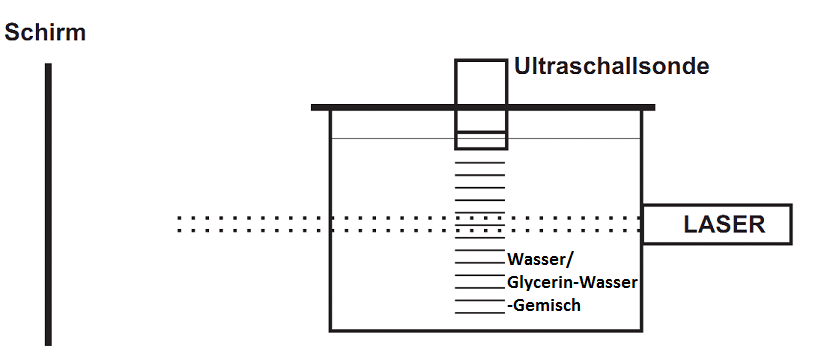
\includegraphics[scale=0.5]{Graphik/Versuchsaufbau}
\caption{Versuchsaufbau$^{\cite{A}}$}
\end{figure}
~\\
Auf eine mit destilliertem Wasser gefüllte Küvette wird eine Ultraschallsonde gesetzt, sodass sich diese blasenfrei unterhalb der Wasseroberfläche befindet. Ein roter Laser mit der Wellenlänge $600$\,nm wird an der Küvette befestigt und ein Schirm wird gegenüber von dem Laser aufgestellt. Der Abstand zwischen Schirm und Küvetten Mitte werden gemessen und notiert.
Der Laser wird eingeschaltet und so reguliert, dass ein paralleler, ausgeweiteter Lichtstrahl auf dem Schirm zu erkennen ist. Die Ultraschallsonde wird angeschaltet, die Frequenz der Sonde wird auf $6$\,MHz gestellt, Strom und Spannungsregler werden aufgedreht und dass Beugungsbild auf dem Schirm wird an der Ultraschallsonde optimiert. Der Laser ist so zu drehen, dass das Bild auf dem Schirm senkrecht steht. Das Strahlenprofil ist nun elliptisch.
Der Versuch ist nun aufgebaut und die Messung kann beginnen. Dazu stellt man die Frequenz der Sonde auf $3$\,MHz ein und misst den Abstand $d_N$ zwischen dem obersten und untersten zu erkennenden Maximums auf dem Schirm. Zudem wird die höchste Beugungsordnung bestimmt. Frequenz, Stromstärke und Widerstand werden zusätzlich notiert.
Diese Messungen werden mit 4 – 12 MHz nacheinander durchgeführt. Darauffolgend führt man einen entsprechenden Versuch mit einem grünen Laser der Wellenlänge $532$\,nm durch. 
Das Glyzerin-Wasser-Gemisch wird auf dieselbe Weise vorbereitet wie das destillierte Wasser. Es wird auch mit einem roten $(600$\,nm) und einem grünen $(532$\,nm) Laser gemessen.

\newpage
\section{ Formeln}

\subsection{Berechnung der Gitterkonstante/Schallwellenlänge}
\begin{equation}
d=\frac{2 \cdot N \cdot \lambda_{\text{Licht}}\cdot a}{d_N}=\lambda_{\text{Schall}}
\label{welle}
\end{equation}
\noindent
$d$: Gitterkonstante;
$N$: Beugungsordnung;
$a$: Abstand zwischen Schirm und Küvette;
$d_N$: Abstand $-N$-ten Beugungsmaximum $+N$-ten Beugungsmaximum;

\subsection{Berechnung der Schallgeschwindigkeit}
\begin{equation}
c=\lambda_{\text{Schall}} \cdot f
\label{Schall}
\end{equation}
\noindent
$c$: Schallgeschwindigkeit;
$\lambda_{\text{Schall}}$: Wellenlänge des Schalls;
$f$: Frequenz der Ultraschallsonde;

\subsection{Berechnung des Kompressionsmodul}

\begin{equation}
K=c_{\text{Schall}}^2 \cdot \rho 
\label{Komp}
\end{equation}
\noindent
$K$: Kompressionsmodul;
$\rho$: Dichte des Mediums;
$c_{\text{Schall}}$: Schallgeschwindigkeit;

\newpage

\section{ Messwerte}

Tabelle 1: 1. Versuch destilliertes Wasser roter Laser ($650$\,nm) \\
\begin{tabular}{|l|c|c|c|c|c|c|c|c|c|c|} \hline
Frequenz $f$ [MHz] & 3 & 4 & 5 & 6 & 7 & 8 & 9 & 10 & 11 & 12\\ \hline
Abstand $d_n$ [mm] & 7 & 15 & 20 & 26 & 21 & 20 & 22 & 28 & 27 & 15 \\ \hline
Beugungsmaximas & 2 & 3 & 4 & 4 & 3 & 2 & 2 & 2 & 2 & 1 \\ \hline 
\end{tabular} \\
~\\
~\\
Tabelle 2: 1. Versuch destilliertes Wasser grüner Laser ($532$\,nm) \\
\begin{tabular}{|l|c|c|c|c|c|c|c|c|c|c|} \hline
Frequenz $f$ [MHz] & 3 & 4 & 5 & 6 & 7 & 8 & 9 & 10 & 11 & 12\\ \hline
Abstand $d_n$ [mm] & 13 & 16 & 20 & 24 & 21 & 24 & 18 & 19 & 11 & 23 \\ \hline
Beugungsmaximas & 4 & 4 & 4 & 4 & 3 & 3 & 2 & 2 & 1 & 2 \\ \hline 
\end{tabular} \\
~\\
~\\
Tabelle 3: 2. Versuch destilliertes Wasser roter Laser ($650$\,nm) \\
\begin{tabular}{|l|c|c|c|c|c|c|c|c|c|c|} \hline
Frequenz $f$ [MHz] & 3 & 4 & 5 & 6 & 7 & 8 & 9 & 10 & 11 & 12\\ \hline
Abstand $d_n$ [mm] & 8 & 15 & 18 & 18 & 19 & 22 & 18 & 20 & 21 & 12 \\ \hline
Beugungsmaximas & 4 & 4 & 4 & 3 & 3 & 3 & 2 & 2 & 2 & 1 \\ \hline 
\end{tabular} \\
~\\
~\\
Tabelle 4: 2. Versuch destilliertes Wasser grüner Laser ($532$\,nm) \\
\begin{tabular}{|l|c|c|c|c|c|c|c|c|c|c|} \hline
Frequenz $f$ [MHz] & 3 & 4 & 5 & 6 & 7 & 8 & 9 & 10 & 11 & 12\\ \hline
Abstand $d_n$ [mm] & 13 & 16 & 26 & 29 & 21 & 24 & 18 & 20 & 22 & 13 \\ \hline
Beugungsmaximas & 4 & 4 & 5 & 5 & 3 & 3 & 2 & 2 & 2 & 1 \\ \hline 
\end{tabular} \\
~\\
~\\
Tabelle 5: 1. Versuch Glyzerin-Wasser-Gemisch roter Laser ($650$\,nm) \\
\begin{tabular}{|l|c|c|c|c|c|c|c|c|c|c|} \hline
Frequenz $f$ [MHz] & 3 & 4 & 5 & 6 & 7 & 8 & 9 & 10 & 11 & 12\\ \hline
Abstand $d_n$ [mm] & 8 & 14 & 16 & 14 & 15 & 9 & 10 & 11 & 12 & 13 \\ \hline
Beugungsmaximas & 2 & 3 & 3 & 2 & 2 & 2 & 1 & 1 & 1 & 1 \\ \hline 
\end{tabular} \\
~\\
~\\
Tabelle 6: 1. Versuch Glyzerin-Wasser-Gemisch grüner Laser ($532$\,nm) \\
\begin{tabular}{|l|c|c|c|c|c|c|c|c|c|c|} \hline
Frequenz $f$ [MHz] & 3 & 4 & 5 & 6 & 7 & 8 & 9 & 10 & 11 & 12\\ \hline
Abstand $d_n$ [mm] & 10 & 15 & 18 & 15 & 13 & 14 & 16 & 18 & 19 & 11 \\ \hline
Beugungsmaximas & 3 & 4 & 4 & 3 & 2 & 2 & 2 & 2 & 2 & 1 \\ \hline 
\end{tabular} \\
~\\
~\\
Tabelle 7: 2. Versuch Glyzerin-Wasser-Gemisch roter Laser ($650$\,nm) \\
\begin{tabular}{|l|c|c|c|c|c|c|c|c|c|c|} \hline
Frequenz $f$ [MHz] & 3 & 4 & 5 & 6 & 7 & 8 & 9 & 10 & 11 & 12\\ \hline
Abstand $d_n$ [mm] & 7 & 14 & 16 & 14 & 15 & 8 & 10 & 11 & 12 & 13 \\ \hline
Beugungsmaximas & 2 & 3 & 3 & 2 & 2 & 1 & 1 & 1 & 1 & 1 \\ \hline 
\end{tabular} \\
~\\
~\\
Tabelle 8: 2. Versuch Glyzerin-Wasser-Gemisch grüner Laser ($532$\,nm) \\
\begin{tabular}{|l|c|c|c|c|c|c|c|c|c|c|} \hline
Frequenz $f$ [MHz] & 3 & 4 & 5 & 6 & 7 & 8 & 9 & 10 & 11 & 12\\ \hline
Abstand $d_n$ [mm] & 12 & 16 & 15 & 17 & 18 & 14 & 15 & 17 & 18 & 10 \\ \hline
Beugungsmaximas & 4 & 4 & 3 & 3 & 3 & 2 & 2 & 2 & 2 & 1 \\ \hline 
\end{tabular}

\newpage
\noindent

\section{ Auswertung}

\subsection{Auswertung der Gitterkonstante/Schallwellenlänge}

Mit Hilfe der Formel (\ref{welle}) können wir die Gitterkonstante $d$ und damit auch die Schallwellenlänge $\lambda_{\text{Schall}}$ berechnen.
Über den gesammten Versuch ist der Wert $\lambda_{\text{Licht}}$ für den roten Laser $650\,$nm, für den grünen $532\,$nm und der Abstand von der Mitte der Küvette zur Wand beträgt $1,38\,$m.  
Eine Beispielrechnung für $N=2$, $d_N= 7\,$mm

\begin{equation*}
d=\frac{2 \cdot N \cdot \lambda_{\text{Licht}}\cdot a}{d_N}=\frac{2 \cdot 2 \cdot 650 \cdot 10^{-9}\,{\text{m}} \cdot 1,38\,{\text{m}}}{0,007\,{\text{m}}}=\lambda_{\text{Schall}} = 51,3\,\text{mm}
\end{equation*}
\noindent
Die Ergebnisse werden in den folgenden Tabellen dargestellt. \\
~\\
Tabelle 9: 1. und 2. Versuch mit Wasser und dem roten Laser. \\
\begin{tabular}{|l|c|c|c|c|c|c|c|c|c|c|} \hline
Abstand $d_n$ [mm] & 7 & 15 & 20 & 26 & 21 & 20 & 22 & 28 & 27 & 15 \\ \hline
Beugungsmaximas & 2 & 3 & 4 & 4 & 3 & 2 & 2 & 2 & 2 & 1 \\ \hline 
Gitterkonstante $d$ [$10^{-4}$\,m] & 5,12 & 3,59 & 3,59 & 2,76 & 2,56 & 1,79 & 1,63 & 1,28 & 1,33 & 1,20 \\ \hline
\end{tabular}\\
\begin{tabular}{|l|c|c|c|c|c|c|c|c|c|c|} \hline
Abstand $d_n$ [mm] & 13 & 16 & 20 & 24 & 21 & 24 & 18 & 19 & 11 & 23 \\ \hline
Beugungsmaximas & 4 & 4 & 4 & 4 & 3 & 3 & 2 & 2 & 1 & 2 \\ \hline 
Gitterkonstante $d$ [$10^{-4}$\,m] & 8,97 & 4,78 & 3,99 & 2,99 & 2,83 & 2,45 & 1,99 & 1,79 & 1,71 & 1,50 \\ \hline 
\end{tabular} \\
~\\
Tabelle 10: 1. und 2. Versuch mit Wasser und dem grünem Laser. \\
\begin{tabular}{|l|c|c|c|c|c|c|c|c|c|c|} \hline
Abstand $d_n$ [mm] & 13 & 16 & 20 & 24 & 21 & 24 & 18 & 19 & 11 & 23 \\ \hline
Beugungsmaximas & 4 & 4 & 4 & 4 & 3 & 3 & 2 & 2 & 1 & 2 \\ \hline 
Gitterkonstante $d$ [$10^{-4}$\,m] & 5,52 & 4,49 & 3,59 & 2,99 & 2,56 & 2,24 & 1,99 & 1,89 & 1,63 & 1,56 \\ \hline 
\end{tabular} \\
\begin{tabular}{|l|c|c|c|c|c|c|c|c|c|c|} \hline
Abstand $d_n$ [mm] & 13 & 16 & 26 & 29 & 21 & 24 & 18 & 20 & 22 & 13 \\ \hline
Beugungsmaximas & 4 & 4 & 5 & 5 & 3 & 3 & 2 & 2 & 2 & 1 \\ \hline 
Gitterkonstante $d$ [$10^{-4}$\,m] & 5,52 & 4,49 & 3,45 & 3,10 & 2,56 & 2,24 & 1,99 & 1,79 & 1,63 & 1,38 \\ \hline 
\end{tabular} \\
~\\
Tabelle 11: 1. und 2. Versuch mit Glycerin- Wasser-Gemisch und dem rotem Laser. \\
\begin{tabular}{|l|c|c|c|c|c|c|c|c|c|c|} \hline
Abstand $d_n$ [mm] & 8 & 14 & 16 & 14 & 15 & 9 & 10 & 11 & 12 & 13 \\ \hline
Beugungsmaximas & 2 & 3 & 3 & 2 & 2 & 2 & 1 & 1 & 1 & 1 \\ \hline 
Gitterkonstante $d$ [$10^{-4}$\,m] &4,49 & 3,84 & 3,36 & 2,56 & 2,39 & 1,99 & 1,79 & 1,63 & 1,50 & 1,38 \\ \hline
\end{tabular} \\
\begin{tabular}{|l|c|c|c|c|c|c|c|c|c|c|} \hline
Abstand $d_n$ [mm] & 7 & 14 & 16 & 14 & 15 & 8 & 10 & 11 & 12 & 13 \\ \hline
Beugungsmaximas & 2 & 3 & 3 & 2 & 2 & 1 & 1 & 1 & 1 & 1 \\ \hline 
Gitterkonstante $d$ [$10^{-4}$\,m] & 5,13 & 3,84 & 3,36 & 2,56 & 2,39 & 2,24 & 1,79 & 1,63 & 1,50 & 1,38 \\ \hline
\end{tabular} \\
~\\
Tabelle 12: 1. und 2. Versuch mit Glycerin- Wasser-Gemisch und dem grünem Laser. \\
\begin{tabular}{|l|c|c|c|c|c|c|c|c|c|c|} \hline
Abstand $d_n$ [mm] & 10 & 15 & 18 & 15 & 13 & 14 & 16 & 18 & 19 & 11 \\ \hline
Beugungsmaximas & 3 & 4 & 4 & 3 & 2 & 2 & 2 & 2 & 2 & 1 \\ \hline 
Gitterkonstante $d$ [$10^{-4}$\,m] & 5,38 & 4,78 & 3,99 & 3,59 & 2,76 & 2,56 & 2,24 & 1,99 &  1,89  & 1,63  \\ \hline
\end{tabular} \\
\begin{tabular}{|l|c|c|c|c|c|c|c|c|c|c|} \hline
Abstand $d_n$ [mm] & 12 & 16 & 15 & 17 & 18 & 14 & 15 & 17 & 18 & 10 \\ \hline
Beugungsmaximas & 4 & 4 & 3 & 3 & 3 & 2 & 2 & 2 & 2 & 1 \\ \hline 
Gitterkonstante $d$ [$10^{-4}$\,m] & 5,98 & 4,49 & 3,59 & 3,17 & 2,99 & 2,56 & 2,39 & 2,11 & 1,99 & 1,79  \\ \hline
\end{tabular}
\newpage

\subsection{Auswertung Schallgeschwindigkeit}

Aus  der Formel (\ref{Schall}) ergibt sich mit Hilfe der Frequenz und der Schallwellenlänge die Schallgeschwindigkeit.\\
Die folgende Beispielrechnung ist für $f=3  \cdot 10^6\,\frac{1}{{\text{s}}}$ und $\lambda_{\text{Schall}}= 51,3$\,mm:
\begin{equation*}
c=\lambda_{\text{Schall}} \cdot f= 5,1257\cdot 10^{-4} \cdot 3 \cdot 10^6\,\frac{1}{{\text{s}}} = 1537,71\,\frac{{\text{m}}}{{\text{s}}}
\end{equation*}
\noindent
Nachfolgend sind die errechneten Werte tabellarisch dargestellt: \\
~\\
Tabelle 13: 1. und 2. Versuch destilliertes Wasser roter Laser  \\
\begin{tabular}{|l|c|c|c|c|c|c|c|c|c|c|} \hline
Frequenz $f$ [MHz] & 3 & 4 & 5 & 6 & 7 \\ \hline
Gitterkonstante $d$ [$10^{-4}$\,m] & 5,12 & 3,59 & 3,59 & 2,76 & 2,56  \\ \hline
Schallgeschwindigkeit $c$ $[\frac{{\text{m}}}{{\text{s}}}]$ & 1537,71 &1435,20 &1794,00 &1656,00 & 1794,00 \\ \hline
Frequenz $f$ [MHz] & 8 & 9 & 10 & 11 & 12\\ \hline
Gitterkonstante $d$ [$10^{-4}$\,m] &  1,79 & 1,63 & 1,28 & 1,33 & 1,20 \\ \hline
Schallgeschwindigkeit $c$ $[\frac{{\text{m}}}{{\text{s}}}]$ & 1435,20 & 1467,82 &1281,43 &1461,78 &1435,20 \\ \hline
\end{tabular} \\
\begin{tabular}{|l|c|c|c|c|c|c|c|c|c|c|} \hline
Frequenz $f$ [MHz] & 3 & 4 & 5 & 6 & 7 \\ \hline
Gitterkonstante $d$ [$10^{-4}$\,m] & 8,97 & 4,78 & 3,99 & 2,99 & 2,83 \\ \hline 
Schallgeschwindigkeit $c$ $[\frac{{\text{m}}}{{\text{s}}}]$ &  2691,00 & 1913,60 & 1993,33 & 1794,00 & 1982,84  \\ \hline
Frequenz $f$ [MHz] &  8 & 9 & 10 & 11 & 12 \\ \hline
Gitterkonstante $d$ [$10^{-4}$\,m] & 2,45 & 1,99 & 1,79 & 1,71 & 1,50 \\ \hline 
Schallgeschwindigkeit $c$ $[\frac{{\text{m}}}{{\text{s}}}]$ & 1957,09 & 1794,00 & 1794,00 & 1879,43 & 1794,00   \\ \hline
\end{tabular} \\
~\\
~\\ 
Tabelle 14: 1. und 2. Versuch destilliertes Wasser grüner Laser \\
\begin{tabular}{|l|c|c|c|c|c|c|c|c|c|c|} \hline
Frequenz $f$ [MHz] & 3 & 4 & 5 & 6 & 7 \\ \hline
Gitterkonstante $d$ [$10^{-4}$\,m] & 5,38 & 4,78 & 3,99 & 3,59 & 2,76  \\ \hline
Schallgeschwindigkeit $c$ $[\frac{{\text{m}}}{{\text{s}}}]$ & 1656,00 & 1794,00 & 1794,00 & 1794,00 & 1794,00 \\ \hline
Frequenz $f$ [MHz] & 8 & 9 & 10 & 11 & 12\\ \hline
Gitterkonstante $d$ [$10^{-4}$\,m] & 2,56 & 2,24 & 1,99 &  1,89  & 1,63  \\ \hline
Schallgeschwindigkeit $c$ $[\frac{{\text{m}}}{{\text{s}}}]$ & 1794,00 &1794,00 & 1888,42 & 1794,00 & 1872,00 \\ \hline
\end{tabular} \\
\begin{tabular}{|l|c|c|c|c|c|c|c|c|c|c|} \hline
Frequenz $f$ [MHz] & 3 & 4 & 5 & 6 & 7 \\ \hline
Gitterkonstante $d$  [$10^{-4}$\,m] & 5,52 & 4,49 & 3,45 & 3,10 & 2,56  \\ \hline 
Schallgeschwindigkeit $c$ $[\frac{{\text{m}}}{{\text{s}}}]$ & 1656,00 & 1794,00 & 1725,00 & 1855,86 & 1794,00   \\ \hline
Frequenz $f$ [MHz]  & 8 & 9 & 10 & 11 & 12\\ \hline
Gitterkonstante $d$ [$10^{-4}$\,m] &  2,24 & 1,99 & 1,79 & 1,63 & 1,38 \\ \hline 
Schallgeschwindigkeit $c$ $[\frac{{\text{m}}}{{\text{s}}}]$ & 1794,00 & 1794,00 & 1794,00 & 1794,00 & 1656,00  \\ \hline
\end{tabular} \\
\newpage
\noindent
Tabelle 15: 1. und 2. Versuch Glyzerin-Wasser-Gemisch roter Laser \\
\begin{tabular}{|l|c|c|c|c|c|c|c|c|c|c|} \hline
Frequenz $f$ [MHz] & 3 & 4 & 5 & 6 & 7 \\ \hline
Gitterkonstante $d$ [$10^{-4}$\,m] & 4,49 & 3,84 & 3,36 & 2,56 & 2,39  \\ \hline
Schallgeschwindigkeit $c$ $[\frac{{\text{m}}}{{\text{s}}}]$ & 1614,60 & 1913,60 & 1993,33 & 2152,80 & 1932,00    \\ \hline
Frequenz $f$ [MHz] & 8 & 9 & 10 & 11 & 12\\ \hline
Gitterkonstante $d$ [$10^{-4}$\,m] & 1,99 & 1,79 & 1,63 & 1,50 & 1,38 \\ \hline
Schallgeschwindigkeit $c$ $[\frac{{\text{m}}}{{\text{s}}}]$ &  2050,29 & 2018,25 & 1993,33 & 2077,26 & 1957,09 \\ \hline
\end{tabular} \\
\begin{tabular}{|l|c|c|c|c|c|c|c|c|c|c|} \hline
Frequenz $f$ [MHz] & 3 & 4 & 5 & 6 & 7 \\ \hline
Gitterkonstante $d$ [$10^{-4}$\,m] & 5,13 & 3,84 & 3,36 & 2,56 & 2,39  \\ \hline
Schallgeschwindigkeit $c$ $[\frac{{\text{m}}}{{\text{s}}}]$ & 1345,50 & 1537,71 & 1681,88 & 1537,71 & 1674,40  \\ \hline
Frequenz $f$ [MHz] &  8 & 9 & 10 & 11 & 12\\ \hline
Gitterkonstante $d$ [$10^{-4}$\,m] &  2,24 & 1,794 & 1,63 & 1,5 & 1,38 \\ \hline
Schallgeschwindigkeit $c$ $[\frac{{\text{m}}}{{\text{s}}}]$ & 1594,67 & 1614,60 & 1630,91 & 1644,50 & 1656,00  \\ \hline
\end{tabular} \\
~\\
~\\
Tabelle 16: 1. und 2. Versuch Glyzerin-Wasser-Gemisch grüner Laser\\
\begin{tabular}{|l|c|c|c|c|c|c|c|c|c|c|} \hline
Frequenz $f$ [MHz] & 3 & 4 & 5 & 6 & 7 \\ \hline
Gitterkonstante $d$ [$10^{-4}$\,m] & 5,38 & 4,78 & 3,99 & 3,59 & 2,76   \\ \hline
Schallgeschwindigkeit $c$ $[\frac{{\text{m}}}{{\text{s}}}]$ & 1614,60 & 1913,60 & 1993,33 & 2152,80 & 1932,00  \\ \hline
Frequenz $f$ [MHz] & 8 & 9 & 10 & 11 & 12\\ \hline
Gitterkonstante $d$ [$10^{-4}$\,m] &  2,56 & 2,24 & 1,99 &  1,89  & 1,63  \\ \hline
Schallgeschwindigkeit $c$ $[\frac{{\text{m}}}{{\text{s}}}]$ & 2050,29 &  2018,25 & 1993,33 & 2077,26 & 1957,09  \\ \hline
\end{tabular} \\
\begin{tabular}{|l|c|c|c|c|c|c|c|c|c|c|} \hline
Frequenz $f$ [MHz] & 3 & 4 & 10 & 11 & 12\\ \hline
Gitterkonstante $d$ [$10^{-4}$\,m] & 5,98 & 4,49 & 3,59 & 3,17 & 2,99   \\ \hline
Schallgeschwindigkeit $c$ $[\frac{{\text{m}}}{{\text{s}}}]$ & 1794,00 & 1794,00 & 1794,00 & 1899,53 & 2093,00   \\ \hline
Frequenz $f$ [MHz] & 8 & 9 & 10 & 11 & 12\\ \hline
Gitterkonstante $d$ [$10^{-4}$\,m] &  2,56 & 2,39 & 2,11 & 1,99 & 1,79  \\ \hline
Schallgeschwindigkeit $c$ $[\frac{{\text{m}}}{{\text{s}}}]$ & 2050,29 & 2152,80 & 2110,59 & 2192,67 & 2152,80  \\ \hline
\end{tabular}\\
\newpage
\noindent
Zu guter Letzt sind noch die Mittelwerte der Schallgeschwindigkeiten zu berechnen, hier Beispielhaft am 1.Versuch mit Wasser und rotem Laser:
\begin{align*}
\bar{c}=\sum_{i=1}^{10} c_i& = 1537,71 \,\frac{{\text{m}}}{{\text{s}}}+ 1435,2 \,\frac{{\text{m}}}{{\text{s}}}+ 1794 \,\frac{{\text{m}}}{{\text{s}}}+ 1656 \,\frac{{\text{m}}}{{\text{s}}}+ 1794\,\frac{{\text{m}}}{{\text{s}}} + 1435,2\,\frac{{\text{m}}}{{\text{s}}}\\ 
&+ 1467,81\,\frac{{\text{m}}}{{\text{s}}} + 1281,43\,\frac{{\text{m}}}{{\text{s}}}  + 1461,78\,\frac{{\text{m}}}{{\text{s}}} + 1435,2\,\frac{{\text{m}}}{{\text{s}}} \\
&= 1529,83\,\frac{{\text{m}}}{{\text{s}}}
\end{align*}
~\\
Die Durchschnittsschallgeschwindigkeiten werden in der nachfolgenden Tabelle aufgelistet:\\
Tabelle 17: Durchschnittsschallgeschwindigkeiten aller Versuche \\
\begin{tabular}{|l|c|} \hline
 & Durchschnittsschallgeschwindigkeit $ \bar{c}~[\frac{{\text{m}}}{{\text{s}}}]$ \\ \hline
  1. Vers. Wasser roter Laser & 1529,83 \\ \hline
  2. Vers. Wasser roter Laser & 1959,33 \\ \hline
  1. Vers. Wasser grüner Laser & 1797,44  \\ \hline
  2. Vers. Wasser grüner Laser & 1765,69 \\ \hline
  1. Vers. Glyzerin-Wasser-Gemisch roter Laser &  1591,79 \\ \hline
  2. Vers. Glyzerin-Wasser-Gemisch roter Laser &1630,94 \\ \hline
  1. Vers. Glyzerin-Wasser-Gemisch grüner Laser & 1970,26 \\ \hline
  2. Vers. Glyzerin-Wasser-Gemisch grüner Laser & 2003,37 \\ \hline
\end{tabular}\\
~\\
\newpage
\noindent
Im Anschluss werden Schallgeschwindigkeit-Frequenz-Diagrammen mit Fehlerbalken eingezeichnet:
\begin{figure}[h]
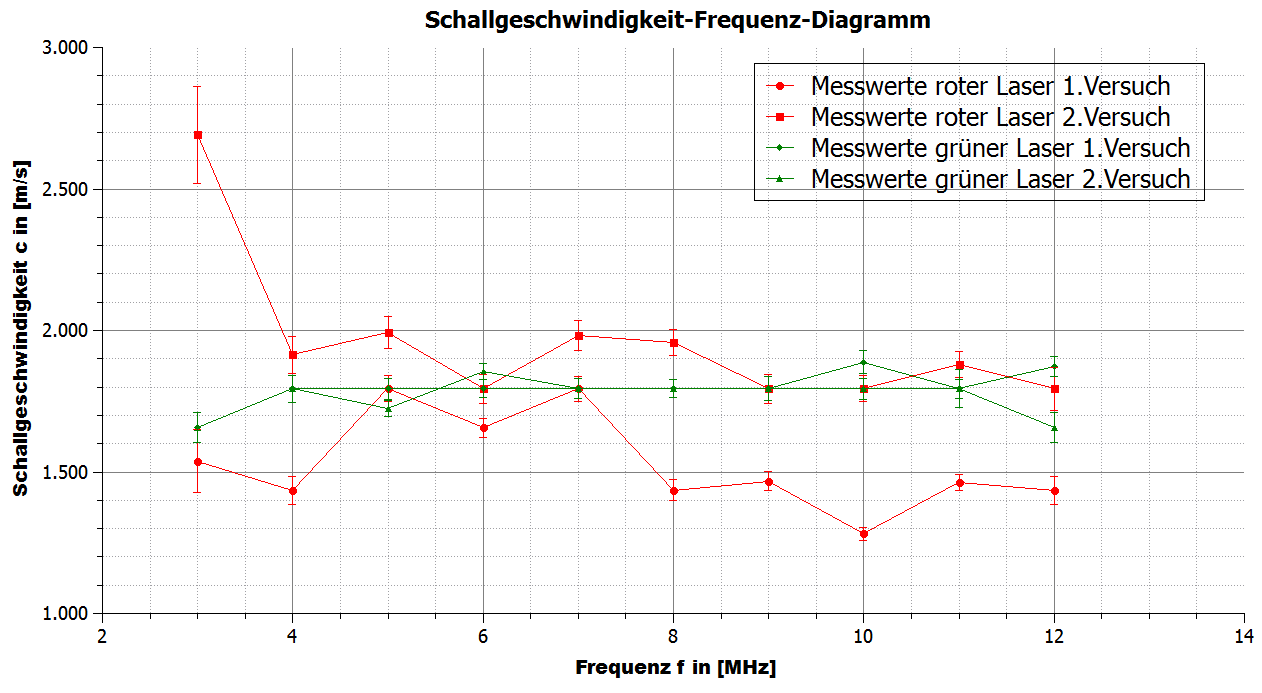
\includegraphics[scale=0.4]{Graphik/SchallgeschwindigkeitWasserFehlerbalken}
\caption{Schallgeschwindigkeitsmessung bei Wasser}
\end{figure}
\noindent
\begin{figure}[h]
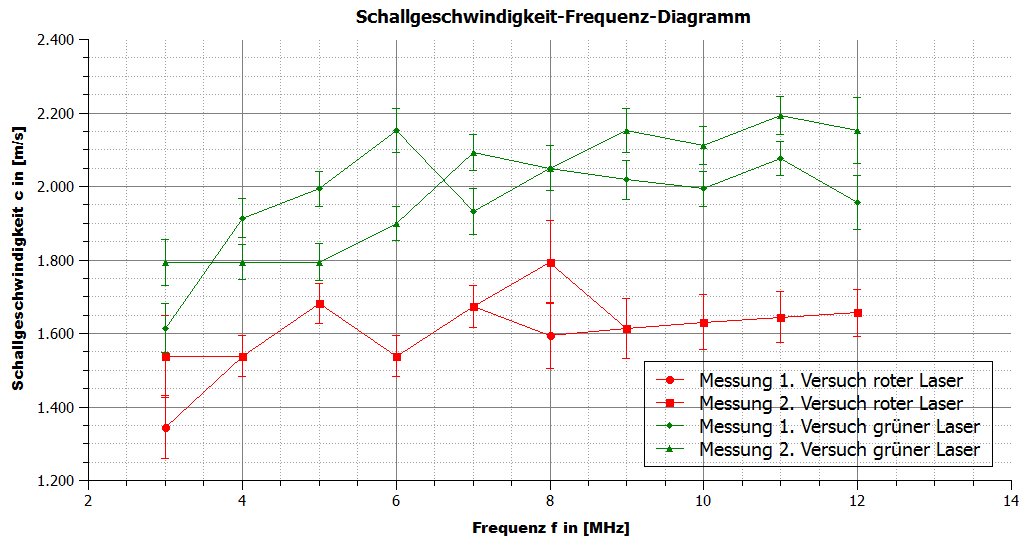
\includegraphics[scale=0.5]{Graphik/SchallgeschwindigkeitGlycerinFehlerbalken}
\caption{Schallgeschwindigkeitsmessung bei Glycerin}
\end{figure}
\newpage
\noindent

\subsection{Auswertung Kompressionsmodul}

Formel (\ref{Komp}) erlaubt nun die Berechnung des Kompressionsmoduls, wobei hier als Dichten jeweils für Wasser $1000\,\frac{{\text{kg}}}{{\text{m}^3}}$ und für Das Glyzerin-Wasser-Gemisch  $1100\,\frac{{\text{kg}}}{{\text{m}^3}}$ angenommen werden.
In der folgenden Beispielrechnung ist das Kompressionsmodul des 1. Versuch mit Wasser bei $3\,{\text{MHz}}$ berechnet worden.
\begin{equation*}
K = \bar{c}^2_{\text{Schall}} \cdot \rho  = 1537,71\,\frac{{\text{m}}}{{\text{s}}} \cdot 1000\,\frac{{\text{kg}}}{{\text{m}^3}}=2,37 \cdot 
10^9\,{\text{Pa}}
\end{equation*}
\noindent
Die Ergebnisse für das Kompressionsmodul sind in den nachfolgenden Tabellen zu entnehmen:\\
~\\
Tabelle 18: 1. Versuch destilliertes Wasser roter Laser  \\
\begin{tabular}{|l|c|c|c|c|c|c|c|c|c|c|} \hline
Schallgeschwindigkeit $c$ $[\frac{{\text{m}}}{{\text{s}}}]$ & 1537,71 &1435,20 &1794,00 &1656,00 & 1794,00 \\ \hline
Kompressionsmodul $K$ [$10^{9}$Pa] & 2,36 & 2,06 & 3,22 & 2,74 & 3,22  \\ \hline
Schallgeschwindigkeit $c$ $[\frac{{\text{m}}}{{\text{s}}}]$ & 1435,20 & 1467,82 &1281,43 &1461,78 &1435,20 \\ \hline
Kompressionsmodul $K$ [$10^9$Pa] & 2,06 & 2,15 & 1,64 & 2,14 & 2,06  \\ \hline
\end{tabular} \\

\newpage
\noindent
Tabelle 19: 1. Versuch destilliertes Wasser grüner Laser \\
\begin{tabular}{|l|c|c|c|c|c|c|c|c|c|c|} \hline
Schallgeschwindigkeit $c$ $[\frac{{\text{m}}}{{\text{s}}}]$ & 1656,00 & 1794,00 & 1794,00 & 1794,00 & 1794,00 \\ \hline
Kompressionsmodul $K$ [$10^9$Pa] &  2,74 & 3,22 & 3,22 & 3,22 & 3,22 \\ \hline
Schallgeschwindigkeit $c$ $[\frac{{\text{m}}}{{\text{s}}}]$ & 1794,00 &1794,00 & 1888,42 & 1794,00 & 1872,00 \\ \hline
Kompressionsmodul $K$ [$10^9$Pa] & 3,22 & 3,22 & 3,57 & 3,22 & 3,50 \\ \hline
\end{tabular} \\

~\\
~\\ 
Tabelle 20: 1. Versuch Glyzerin-Wasser-Gemisch roter Laser \\
\begin{tabular}{|l|c|c|c|c|c|c|c|c|c|c|} \hline
Schallgeschwindigkeit $c$ $[\frac{{\text{m}}}{{\text{s}}}]$ & 1614,60 & 1913,60 & 1993,33 & 2152,80 & 1932,00    \\ \hline
Kompressionsmodul $K$ [$10^9$Pa] & 1,99 & 2,60 & 3,11 & 2,60 & 3,08  \\ \hline
Schallgeschwindigkeit $c$ $[\frac{{\text{m}}}{{\text{s}}}]$ &  2050,29 & 2018,25 & 1993,33 & 2077,26 & 1957,09 \\ \hline
Kompressionsmodul $K$ [$10^9$Pa] & 2,80 & 2,87 & 2,93 & 2,97 & 3,02 \\ \hline
\end{tabular} \\

~\\
~\\
Tabelle 21: 1. Versuch Glyzerin-Wasser-Gemisch grüner Laser\\
\begin{tabular}{|l|c|c|c|c|c|c|c|c|c|c|} \hline
Schallgeschwindigkeit $c$ $[\frac{{\text{m}}}{{\text{s}}}]$ & 1614,60 & 1913,60 & 1993,33 & 2152,80 & 1932,00  \\ \hline
Kompressionsmodul $K$ [$10^9$Pa] & 2,87 & 4,03 & 4,37 & 5,10 & 4,11  \\ \hline
Schallgeschwindigkeit $c$ $[\frac{{\text{m}}}{{\text{s}}}]$ & 2050,29 &  2018,25 & 1993,33 & 2077,26 & 1957,09  \\ \hline
Kompressionsmodul $K$ [$10^9$Pa]  & 4,62 & 4,48 & 4,37 & 4,75 & 4,21  \\ \hline
\end{tabular} \\

\newpage

\section{Fehlerrechnung}

\subsection{Fehlerquellen}

Dieser Versuch hat neben den üblichen Mess- und Ableseungenauigkeiten zwei besondere Fehlerquellen, zum einen ist es nur bedingt möglich, die Ultraschallsonde so zu platzieren, dass sie völlig blasenfrei unter der Wasseroberfläche liegt. Eine andere Fehlerquelle ist bei dem Ablesen der Beugungsordnung zu finden. Der Versuchsraum war sehr hell und ein Justieren des Lasers half nur bedingt, weswegen das Übersehen einer Beugungsordnung durchaus ebenfalls passieren kann. Da diese Fehler nicht quantitativ erfasst werden könne, sind auch keine Aussagen über Größe und Auswirkung dieser Fehler möglich. Die Messungenauigkeiten in diesem Versuch sind erstens bei Messen von $d_N$ und zweitens beim Messen von $N$, welche mit einer Fehlertoleranz von $\Delta d_N = 0,05\,\text{mm}$ und $\Delta a= 1\,{\text{mm}}$ mitberechnet werden.

\subsection{Fehler bei der Gitterkonstante /Schallwellenlänge}
Anhand eine Beispielrechnung wird noch erklärt, wie die Fehlerberechnung erfolgt. Diese Beispielrechnung ist über den 1.Versuch Im Anschluss werden alle Ergebnisse in einer Tabelle zusammengefasst. \\
\begin{align*}
\Delta d &=  \vert \frac{2 \cdot N \cdot \lambda_{\text{Licht}}\cdot \Delta a}{d_N}\vert 
+ \vert - \frac{2 \cdot N \cdot \lambda_{\text{Licht}}\cdot \Delta a}{d^2_N}\vert \\
&= \vert\frac{2 \cdot 2 \cdot 650 \cdot 10^{-9}\,{\text{m}} \cdot  0,001\,{\text{m}}}{0,007\,{\text{m}}} \vert 
+ \vert \frac{2 \cdot 2 \cdot 650 \cdot 10^{-9}\,{\text{m}} \cdot  1,38\,{\text{m}}}{0,0005\,{\text{m}}} \vert \\
&= 5,13 \,\text{mm}
\end{align*}
\newpage
\noindent
Tabelle 22: 1. Versuch mit Wasser und dem roten Laser. \\
\begin{tabular}{|l|c|c|c|c|c|c|c|c|c|c|} \hline
Abstand $d_n$ [mm] & 7 & 15 & 20 & 26 & 21 & 20 & 22 & 28 & 27 & 15 \\ \hline
Beugungsmaximas & 2 & 3 & 4 & 4 & 3 & 2 & 2 & 2 & 2 & 1 \\ \hline 
Gitterkonstante $d$ [$10^{-4}$\,m] & 5,12 & 3,59 & 3,59 & 2,76 & 2,56 & 1,79 & 1,63 & 1,28 & 1,33 & 1,20 \\ \hline
Fehler $\Delta d$ [$10^{-6}$\,m] & 36,98 & 12,22 & 9,23 & 5,51 & 6,29 & 4,62 & 3,82 & 2,38 &  2,56 & 4,07  \\ \hline
\end{tabular}\\

~\\
Tabelle 23: 1. Versuch mit Wasser und dem grünem Laser. \\
\begin{tabular}{|l|c|c|c|c|c|c|c|c|c|c|} \hline
Abstand $d_n$ [mm] & 13 & 16 & 20 & 24 & 21 & 24 & 18 & 19 & 11 & 23 \\ \hline
Beugungsmaximas & 4 & 4 & 4 & 4 & 3 & 3 & 2 & 2 & 1 & 2 \\ \hline 
Gitterkonstante $d$ [$10^{-4}$\,m] & 5,52 & 4,49 & 3,59 & 2,99 & 2,56 & 2,24 & 1,99 & 1,89 & 1,63 & 1,56 \\ \hline 
Fehler $\Delta d$ [$10^{-6}$\,m]  & 17,70 & 11,74 & 7,55  & 5,28 & 5,15 & 3,96 & 4,65 & 4,18 & 6,16 & 2,87 \\ \hline
\end{tabular} \\

~\\
Tabelle 24: 1. Versuch mit Glycerin- Wasser-Gemisch und dem rotem Laser. \\
\begin{tabular}{|l|c|c|c|c|c|c|c|c|c|c|} \hline
Abstand $d_n$ [mm] & 8 & 14 & 16 & 14 & 15 & 9 & 10 & 11 & 12 & 13 \\ \hline
Beugungsmaximas & 2 & 3 & 3 & 2 & 2 & 2 & 1 & 1 & 1 & 1 \\ \hline 
Gitterkonstante $d$ [$10^{-4}$\,m] &4,49 & 3,84 & 3,36 & 2,56 & 2,39 & 1,99 & 1,79 & 1,63 & 1,50 & 1,38 \\ \hline
Fehler $\Delta d$ [$10^{-6}$\,m]  &  28,36 & 14,01 & 10,76 & 9,34 & 8,15 & 11,22 & 9,10 & 7,53 & 6,34 & 5,41 \\ \hline
\end{tabular} \\

~\\
Tabelle 25: 1. Versuch mit Glycerin- Wasser-Gemisch und dem grünem Laser. \\
\begin{tabular}{|l|c|c|c|c|c|c|c|c|c|c|} \hline
Abstand $d_n$ [mm] & 10 & 15 & 18 & 15 & 13 & 14 & 16 & 18 & 19 & 11 \\ \hline
Beugungsmaximas & 3 & 4 & 4 & 3 & 2 & 2 & 2 & 2 & 2 & 1 \\ \hline 
Gitterkonstante $d$ [$10^{-4}$\,m] & 5,38 & 4,78 & 3,99 & 3,59 & 2,76 & 2,56 & 2,24 & 1,99 &  1,89  & 1,63  \\ \hline
Fehler $\Delta d$ [$10^{-6}$\,m]  & 22,34 & 13,34  & 9,30 & 10,00 & 8,85 & 7,64 & 5,87 & 4,65 & 4,18 & 6,16  \\ \hline
\end{tabular} \\

\newpage

\subsection{Fehler bei der Schallgeschwindigkeit}

Mit Hilfe einer Beispielrechnung soll nochmal verdeutlicht werden, wie die Fehlertoleranz bei der Schallgeschwindigkeit errechnet wird.
Auch hier wird wieder der 1. Versuch mit Wasser und dem roten Laser verwendet. Im Anschluss werden alle errechneten Fehlertoleranzen in einer Tabelle zusammengefasst.
\begin{align*}
\Delta c=\vert \Delta \lambda_{\text{Schall}} \cdot f \vert = \vert 36,98 \cdot 10^{-6}\,{\text{m}} \cdot 3\cdot 1000000\,\frac{1}{{\text{s}}} \vert =110,95\,\frac{{\text{m}}}{{\text{s}}}
\end{align*}
\noindent
Tabelle 26: 1. Versuch destilliertes Wasser roter Laser  \\
\begin{tabular}{|l|c|c|c|c|c|c|c|c|c|c|} \hline
Frequenz $f$ [MHz] & 3 & 4 & 5 & 6 & 7 \\ \hline
Gitterkonstante $d$ [$10^{-4}$\,m] & 5,12 & 3,59 & 3,59 & 2,76 & 2,56  \\ \hline
Schallgeschwindigkeit $c$ $[\frac{{\text{m}}}{{\text{s}}}]$ & 1537,71 &1435,20 &1794,00 &1656,00 & 1794,00 \\ \hline
Fehler Schallgeschwindigkeit $\Delta c$ $[\frac{{\text{m}}}{{\text{s}}}]$ & 110,95 &
48,88 &
46,15 &
33,05 &
44,01 \\ \hline
Frequenz $f$ [MHz] & 8 & 9 & 10 & 11 & 12\\ \hline
Gitterkonstante $d$ [$10^{-4}$\,m] &  1,79 & 1,63 & 1,28 & 1,33 & 1,20 \\ \hline
Schallgeschwindigkeit $c$ $[\frac{{\text{m}}}{{\text{s}}}]$ & 1435,20 & 1467,82 &1281,43 &1461,78 &1435,20 \\ \hline
Fehler Schallgeschwindigkeit $\Delta c$ $[\frac{{\text{m}}}{{\text{s}}}]$ & 36,92 &
34,42 &
23,81 &
28,13 &
48,88  \\ \hline
\end{tabular} \\

~\\
~\\ 
Tabelle 27: 1. Versuch destilliertes Wasser grüner Laser \\
\begin{tabular}{|l|c|c|c|c|c|c|c|c|c|c|} \hline
Frequenz $f$ [MHz] & 3 & 4 & 5 & 6 & 7 \\ \hline
Gitterkonstante $d$ [$10^{-4}$\,m] & 5,38 & 4,78 & 3,99 & 3,59 & 2,76  \\ \hline
Schallgeschwindigkeit $c$ $[\frac{{\text{m}}}{{\text{s}}}]$ & 1656,00 & 1794,00 & 1794,00 & 1794,00 & 1794,00 \\ \hline
Fehler Schallgeschwindigkeit $\Delta c$ $[\frac{{\text{m}}}{{\text{s}}}]$ & 53,11 & 
46,95 & 
37,77 & 
31,65 & 
36,02 
 \\ \hline
Frequenz $f$ [MHz] & 8 & 9 & 10 & 11 & 12\\ \hline
Gitterkonstante $d$ [$10^{-4}$\,m] & 2,56 & 2,24 & 1,99 &  1,89  & 1,63  \\ \hline
Schallgeschwindigkeit $c$ $[\frac{{\text{m}}}{{\text{s}}}]$ & 1794,00 &1794,00 & 1888,42 & 1794,00 & 1872,00 \\ \hline
Fehler Schallgeschwindigkeit $\Delta c$ $[\frac{{\text{m}}}{{\text{s}}}]$ & 
31,65 & 
41,85 & 
41,79 & 
67,81 & 
34,42  \\ \hline
\end{tabular} \\

\newpage
\noindent
Tabelle 28: 1. Versuch Glyzerin-Wasser-Gemisch roter Laser \\
\begin{tabular}{|l|c|c|c|c|c|c|c|c|c|c|} \hline
Frequenz $f$ [MHz] & 3 & 4 & 5 & 6 & 7 \\ \hline
Gitterkonstante $d$ [$10^{-4}$\,m] & 4,49 & 3,84 & 3,36 & 2,56 & 2,39  \\ \hline
Schallgeschwindigkeit $c$ $[\frac{{\text{m}}}{{\text{s}}}]$ & 1614,60 & 1913,60 & 1993,33 & 2152,80 & 1932,00    \\ \hline
Fehler Schallgeschwindigkeit $\Delta c$ $[\frac{{\text{m}}}{{\text{s}}}]$ & 85,07 & 
56,03 & 
53,78 & 
56,03 & 
57,03 
  \\ \hline
Frequenz $f$ [MHz] & 8 & 9 & 10 & 11 & 12\\ \hline
Gitterkonstante $d$ [$10^{-4}$\,m] & 1,99 & 1,79 & 1,63 & 1,50 & 1,38 \\ \hline
Schallgeschwindigkeit $c$ $[\frac{{\text{m}}}{{\text{s}}}]$ &  2050,29 & 2018,25 & 1993,33 & 2077,26 & 1957,09 \\ \hline
Fehler Schallgeschwindigkeit $\Delta c$ $[\frac{{\text{m}}}{{\text{s}}}]$ & 
89,75 & 
81,90 & 
75,31 & 
69,71 & 
64,89  \\ \hline
\end{tabular} \\

~\\
~\\
Tabelle 29: 1. Versuch Glyzerin-Wasser-Gemisch grüner Laser\\
\begin{tabular}{|l|c|c|c|c|c|c|c|c|c|c|} \hline
Frequenz $f$ [MHz] & 3 & 4 & 5 & 6 & 7 \\ \hline
Gitterkonstante $d$ [$10^{-4}$\,m] & 5,38 & 4,78 & 3,99 & 3,59 & 2,76   \\ \hline
Schallgeschwindigkeit $c$ $[\frac{{\text{m}}}{{\text{s}}}]$ & 1614,60 & 1913,60 & 1993,33 & 2152,80 & 1932,00  \\ \hline
Fehler Schallgeschwindigkeit $\Delta c$ $[\frac{{\text{m}}}{{\text{s}}}]$ & 67,03 & 
53,34  & 
46,50 & 
60,01 & 
61,96 
 \\ \hline
Frequenz $f$ [MHz] & 8 & 9 & 10 & 11 & 12\\ \hline
Gitterkonstante $d$ [$10^{-4}$\,m] &  2,56 & 2,24 & 1,99 &  1,89  & 1,63  \\ \hline
Schallgeschwindigkeit $c$ $[\frac{{\text{m}}}{{\text{s}}}]$ & 2050,29 &  2018,25 & 1993,33 & 2077,26 & 1957,09  \\ \hline
Fehler Schallgeschwindigkeit $\Delta c$ $[\frac{{\text{m}}}{{\text{s}}}]$ & 
61,15 & 
52,82 & 
46,50 & 
45,97 & 
73,97 \\ \hline
\end{tabular} \\


\subsection{Fehler beim Kompressionsmodul}

Hier wird ebenfalls an Hand einer Beispielrechnung für den ersten Versuch mit Wasser und dem roten Laser klargemacht, wie die Fehlerberechnung funktioniert. Folgend werden die Ergebnisse dann in die Tabelle eingetragen.
\begin{equation*}
\Delta K=\vert 2\cdot \bar{c}_{\text{Schall}} \cdot \rho \cdot \Delta c \vert = 2\cdot  1000\,\frac{{\text{kg}}}{{\text{m}^3}}\cdot1529,83\,\frac{{\text{m}}}{{\text{s}}}\cdot 110,95\,\frac{{\text{m}}}{{\text{s}}} = 339473264,50\,{\text{Pa}}
\end{equation*}
\noindent
Tabelle 30: 1. Versuch destilliertes Wasser roter Laser  \\
\begin{tabular}{|l|c|c|c|c|c|c|c|c|c|c|} \hline
$K$ [$10^9$Pa] & 2,36 & 2,06 & 3,22 & 2,74 & 3,22  \\ \hline
Fehler $\Delta K$ [$10^9$Pa] & 3,39 &
1,50 & 
1,41 & 
1,01 & 
1,35 
  \\ \hline
$K$ [$10^9$Pa] & 2,06 & 2,15 & 1,64 & 2,14 & 2,06  \\ \hline
Fehler $\Delta K$ [Pa] & 
1,13 & 
1,05 & 
7,29 & 
8,61 & 
1,50 \\ \hline
\end{tabular} \\

~\\
~\\ 
Tabelle 31: 1. Versuch destilliertes Wasser grüner Laser \\
\begin{tabular}{|l|c|c|c|c|c|c|c|c|c|c|} \hline
 $K$ [$10^9$Pa] & 2,74 & 3,22 & 2,98 & 3,44 & 3,22   \\ \hline
Fehler  $\Delta K$ [$10^9$Pa] & 1,90930979,11 & 
1,69 & 
1,36 & 
1,14 & 
1,30  \\ \hline
 $K$ [$10^9$Pa] & 3,22 & 3,22 & 3,22 & 3,22 & 2,74   \\ \hline
Fehler  $\Delta K$ [$10^9$Pa] &  1,14 & 
1,50 & 
1,50 & 
2,44 & 
1,24 
\\ \hline 
\end{tabular} \\

\newpage
Tabelle 32: 1. Versuch Glyzerin-Wasser-Gemisch roter Laser \\
\begin{tabular}{|l|c|c|c|c|c|c|c|c|c|c|} \hline
 $K$ [$10^9$Pa] & 1,99 & 2,60 & 3,11 & 2,60 & 3,08  \\ \hline
Fehler $\Delta K$ [$10^9$Pa] &  2,98  & 
1,96 & 
1,88 & 
1,96 & 
2,00
\\ \hline
 $K$ [$10^9$Pa] & 2,80 & 2,87 & 2,93 & 2,97 & 3,02 \\ \hline
Fehler $\Delta K$ [$10^9$Pa] & 3,14 & 
2,87 & 
2,64 & 
2,44 & 
2,27
  \\ \hline
\end{tabular} \\

~\\
~\\
Tabelle 33: 1. Versuch Glyzerin-Wasser-Gemisch grüner Laser\\
\begin{tabular}{|l|c|c|c|c|c|c|c|c|c|c|} \hline
 $K$ [$10^9$Pa] & 2,87 & 4,03 & 4,37 & 5,10 & 4,11  \\ \hline
Fehler $\Delta K$ [$10^9$Pa] & 2,91  & 
2,31 & 
2,02 & 
2,60 & 
2,69
 \\ \hline
 $K$ [$10^9$Pa]  & 4,62 & 4,48 & 4,3 & 4,75 & 4,21  \\ \hline
Fehler $\Delta K$ [$10^9$Pa] &  2,65 & 
2,29 & 
2,02 & 
2,00 & 
3,21
\\ \hline
\end{tabular} \\


\section{Zusammenfassung}

Im Versuch wurden die Schallgeschwindigkeit, Schallwellenlänge und das Kompressionsmodul mit Fehlertoleranzen in Wasser und einem Glyzerin-Wasser-
Gemisch errechnet werden . Aus der Literatur wissen wir, dass die Schreitgeschwindigkeit bei  $25^{\circ}\,C$ warmen destilliertem Wasser etwa $1497 \frac{{\text{m}}}{{\text{s}}}$ und für Glyzerin bei $20^{\circ}\,C$ etwa $1923 \frac{{\text{m}}}{{\text{s}}}$  liegt.$^{\cite{2}}$
Die Durchschnittsschallgeschwindigkeit im ersten Versuchsdurchgang sind wir mit dem roten Laser im destilliertem Wasser dem Literaturwert von destilliertem Wasser am nächsten. 
Wohingegen die Durchschnittsschallgeschwindigkeit der erste Durchgang mit dem grünen Laser im Glyzerin-Wasser-Gemisch dem Literaturwert von Glyzerin am nächsten ist.
Bei den Kompressionsmodulen liegt der Literaturwert für $20^{\circ}C$ bei Wasser bei etwa $2,1 \cdot 10^9\, \text{Pa}$ und bei Glyzerin bei etwa $4,7 \cdot 10^9\, \text{Pa}$.$^{\cite{3}}$ Wieder sind wir bei Wasser mit rotem Laser im ersten Durchgang dem Literaturwert im Schnitt am nächsten ($\bar{K}=(2,37\pm 0,34)\, \text{$\cdot 10^9$Pa}$) und dem ersten Versuch mit grünem Laser im Glyzerin-Wasser-Gemisch dem Literaturwert für Glyzerin im Schnitt am nächsten ($\bar{K}=(4,45\pm 0,29)\, \text{$\cdot 10^9$Pa}$). \\
\newpage
\noindent
Zu guter Letzt  werden hier nochmal alle Ergebnisse samt Fehlertoleranz tabellarisch angegeben: \\
~\\
Tabelle 34: 1. Versuch mit Wasser und dem roten Laser. \\
\begin{tabular}{|l|c|c|c|c|c|c|c|c|c|c|} \hline
Gitterkonstante $d$ [$10^{-4}$\,m] & 5,12 & 3,59 & 3,59 & 2,76 & 2,56 & 1,79 & 1,63 & 1,28 & 1,33 & 1,20 \\ \hline
Fehler $\Delta d$ [$10^{-6}$\,m] & 36,98 & 12,22 & 9,23 & 5,51 & 6,29 & 4,62 & 3,82 & 2,38 &  2,56 & 4,07  \\ \hline
\end{tabular}\\

~\\
Tabelle 35: 1. Versuch mit Wasser und dem grünem Laser. \\
\begin{tabular}{|l|c|c|c|c|c|c|c|c|c|c|} \hline
Gitterkonstante $d$ [$10^{-4}$\,m] & 5,52 & 4,49 & 3,59 & 2,99 & 2,56 & 2,24 & 1,99 & 1,89 & 1,63 & 1,56 \\ \hline 
Fehler $\Delta d$ [$10^{-6}$\,m]  & 17,70 & 11,74 & 7,55  & 5,28 & 5,15 & 3,96 & 4,65 & 4,18 & 6,16 & 2,87 \\ \hline
\end{tabular} \\

~\\
Tabelle 36: 1. Versuch mit Glycerin- Wasser-Gemisch und dem rotem Laser. \\
\begin{tabular}{|l|c|c|c|c|c|c|c|c|c|c|} \hline
Gitterkonstante $d$ [$10^{-4}$\,m] &4,49 & 3,84 & 3,36 & 2,56 & 2,39 & 1,99 & 1,79 & 1,63 & 1,50 & 1,38 \\ \hline
Fehler $\Delta d$ [$10^{-6}$\,m]  &  28,36 & 14,01 & 10,76 & 9,34 & 8,15 & 11,22 & 9,10 & 7,53 & 6,34 & 5,41 \\ \hline
\end{tabular} \\

~\\
Tabelle 37: 1. Versuch mit Glycerin- Wasser-Gemisch und dem grünem Laser. \\
\begin{tabular}{|l|c|c|c|c|c|c|c|c|c|c|} \hline
Gitterkonstante $d$ [$10^{-4}$\,m] & 5,38 & 4,78 & 3,99 & 3,59 & 2,76 & 2,56 & 2,24 & 1,99 &  1,89  & 1,63  \\ \hline
Fehler $\Delta d$ [$10^{-6}$\,m]  & 22,34 & 13,34  & 9,30 & 10,00 & 8,85 & 7,64 & 5,87 & 4,65 & 4,18 & 6,16  \\ \hline
\end{tabular} \\

~\\
~\\
Tabelle 38: 1. Versuch destilliertes Wasser roter Laser  \\
\begin{tabular}{|l|c|c|c|c|c|c|c|c|c|c|} \hline
Schallgeschwindigkeit $c$ $[\frac{{\text{m}}}{{\text{s}}}]$ & 1537,71 &1435,20 &1794,00 &1656,00 & 1794,00 \\ \hline
Fehler Schallgeschwindigkeit $\Delta c$ $[\frac{{\text{m}}}{{\text{s}}}]$ & 110,95 &
48,88 &
46,15 &
33,05 &
44,01 
 \\ \hline
Schallgeschwindigkeit $c$ $[\frac{{\text{m}}}{{\text{s}}}]$ & 1435,20 & 1467,82 &1281,43 &1461,78 &1435,20 \\ \hline
Fehler Schallgeschwindigkeit $\Delta c$ $[\frac{{\text{m}}}{{\text{s}}}]$ & 36,92 &
34,42 &
23,81 &
28,13 &
48,88  \\ \hline
\end{tabular} \\

~\\
~\\ 
Tabelle 39: 1. Versuch destilliertes Wasser grüner Laser \\
\begin{tabular}{|l|c|c|c|c|c|c|c|c|c|c|} \hline
Schallgeschwindigkeit $c$ $[\frac{{\text{m}}}{{\text{s}}}]$ & 1656,00 & 1794,00 & 1794,00 & 1794,00 & 1794,00 \\ \hline
Fehler Schallgeschwindigkeit $\Delta c$ $[\frac{{\text{m}}}{{\text{s}}}]$ & 53,11 & 
46,95 & 
37,77 & 
31,65 & 
36,02 
 \\ \hline
Schallgeschwindigkeit $c$ $[\frac{{\text{m}}}{{\text{s}}}]$ & 1794,00 &1794,00 & 1888,42 & 1794,00 & 1872,00 \\ \hline
Fehler Schallgeschwindigkeit $\Delta c$ $[\frac{{\text{m}}}{{\text{s}}}]$ & 
31,65 & 
41,85 & 
41,79 & 
67,81 & 
34,42  \\ \hline
\end{tabular} \\

~\\
~\\
Tabelle 40: 1. Versuch Glyzerin-Wasser-Gemisch roter Laser \\
\begin{tabular}{|l|c|c|c|c|c|c|c|c|c|c|} \hline
Schallgeschwindigkeit $c$ $[\frac{{\text{m}}}{{\text{s}}}]$ & 1614,60 & 1913,60 & 1993,33 & 2152,80 & 1932,00    \\ \hline
Fehler Schallgeschwindigkeit $\Delta c$ $[\frac{{\text{m}}}{{\text{s}}}]$ & 85,07 & 
56,03 & 
53,78 & 
56,03 & 
57,03 
  \\ \hline
Schallgeschwindigkeit $c$ $[\frac{{\text{m}}}{{\text{s}}}]$ &  2050,29 & 2018,25 & 1993,33 & 2077,26 & 1957,09 \\ \hline
Fehler Schallgeschwindigkeit $\Delta c$ $[\frac{{\text{m}}}{{\text{s}}}]$ & 
89,75 & 
81,90 & 
75,31 & 
69,71 & 
64,89  \\ \hline
\end{tabular} \\

~\\
~\\
Tabelle 41: 1. Versuch Glyzerin-Wasser-Gemisch grüner Laser\\
\begin{tabular}{|l|c|c|c|c|c|c|c|c|c|c|} \hline
Schallgeschwindigkeit $c$ $[\frac{{\text{m}}}{{\text{s}}}]$ & 1614,60 & 1913,60 & 1993,33 & 2152,80 & 1932,00  \\ \hline
Fehler Schallgeschwindigkeit $\Delta c$ $[\frac{{\text{m}}}{{\text{s}}}]$ & 67,03 & 
53,34  & 
46,50 & 
60,01 & 
61,96 
 \\ \hline
Schallgeschwindigkeit $c$ $[\frac{{\text{m}}}{{\text{s}}}]$ & 2050,29 &  2018,25 & 1993,33 & 2077,26 & 1957,09  \\ \hline
Fehler Schallgeschwindigkeit $\Delta c$ $[\frac{{\text{m}}}{{\text{s}}}]$ & 
61,15 & 
52,82 & 
46,50 & 
45,97 & 
73,97 \\ \hline
\end{tabular} \\

~\\
~\\
Tabelle 42: 1. Versuch destilliertes Wasser roter Laser  \\
\begin{tabular}{|l|c|c|c|c|c|c|c|c|c|c|} \hline
$K$ [$10^9$Pa] & 2,36 & 2,06 & 3,22 & 2,74 & 3,22  \\ \hline
Fehler $\Delta K$ [$10^9$Pa] & 3,40 &
1,50 & 
1,41 & 
1,01 & 
1,35 
  \\ \hline
$K$ [$10^9$Pa] & 2,06 & 2,15 & 1,64 & 2,14 & 2,06  \\ \hline
Fehler $\Delta K$ [$10^9$Pa] & 
1,13 & 
1,05 & 
7,29 & 
8,61 & 
1,50 \\ \hline
\end{tabular} \\

~\\
~\\ 
Tabelle 43: 1. Versuch destilliertes Wasser grüner Laser \\
\begin{tabular}{|l|c|c|c|c|c|c|c|c|c|c|} \hline
 $K$ [$10^9$Pa] & 2,74 & 3,22 & 2,98 & 3,44 & 3,22   \\ \hline
Fehler  $\Delta K$ [$10^9$Pa] & 1,91 & 
1,69 & 
1,36 & 
1,14 & 
1,30  \\ \hline
 $K$ [$10^9$Pa] & 3,22 & 3,22 & 3,22 & 3,22 & 2,74   \\ \hline
Fehler  $\Delta K$ [$10^9$Pa] &  1,14 & 
1,50 & 
1,50 & 
2,44 & 
1,24 
\\ \hline 
\end{tabular} \\

~\\
~\\ 
Tabelle 44: 1. Versuch Glyzerin-Wasser-Gemisch roter Laser \\
\begin{tabular}{|l|c|c|c|c|c|c|c|c|c|c|} \hline
 $K$ [$10^9$Pa] & 1,991407275 & 2,60 & 3,11 & 2,60 & 3,08  \\ \hline
Fehler $\Delta K$ [$10^9$Pa] &  2,98  & 
1,96 & 
1,88 & 
1,96 & 
2,00
\\ \hline

 $K$ [$10^9$Pa] & 2,80 & 2,87 & 2,93 & 2,97 & 3,02 \\ \hline
Fehler $\Delta K$ [$10^9$Pa] & 3,14 & 
2,87 & 
2,64 & 
2,44 & 
2,27
  \\ \hline
\end{tabular} \\

~\\
~\\
Tabelle 45: 1. Versuch Glyzerin-Wasser-Gemisch grüner Laser\\
\begin{tabular}{|l|c|c|c|c|c|c|c|c|c|c|} \hline

 $K$ [$10^9$Pa] & 2,87 & 4,03 & 4,37 & 5,10 & 4,11  \\ \hline
Fehler $\Delta K$ [$10^9$Pa] & 2,91  & 
2,31 & 
2,02 & 
2,60 & 
2,69
 \\ \hline
 $K$ [$10^9$Pa]  & 4,62 & 4,48 & 4,37 & 4,75 & 4,21  \\ \hline
Fehler $\Delta K$ [$10^9$Pa] &  2,65 & 
2,29 & 
2,02 & 
1,99 & 
3,21
\\ \hline
\end{tabular} \\


\section{Literaturverzeichnis}

\begin{thebibliography}{xxxxxxxx}
	\bibitem[1]{1}	\textit{\glqq S12 Ultraschallwellen nach Debye-Sears\grqq , in http://www3.physik.uni-stuttgart.de/studium/praktika/ap/},\textit{ unter 										http://www3.physik.uni-stuttgart.de/studium/praktika/ap/pdf\_dateien/S12.pdf abgerufen am 21.05.2015}
   \bibitem[2]{2} \textit{\glqq Dichte, Schallgeschwindigkeit transversal und longitudinal, akust.Impendanz\grqq, in http://www.flowanalytic.com unter 
                          http://www.flowanalytic.com/schall.pdf" abgerufen am 21.05.2015}
   \bibitem[3]{3}  H. Hammer, K.Hammer, \textit{ Grundkurs der Physik 1: Mechanik - Wärmelehre}, Walter de Gruyter, Berlin,~\textbf{1995}, S.107 				                           Tabelle 3.1-1
    \bibitem[A]{A}  Graphik aus \textit{\glqq S12 Ultraschallwellen nach Debye-Sears\grqq , in http://www3.physik.uni-stuttgart.de/studium/praktika/ap/},											\textit{ unter 	http://www3.physik.uni-stuttgart.de/studium/praktika/ap/pdf\_dateien/S12.pdf abgerufen am 21.05.2015}
\end{thebibliography}
\newpage

\begin{figure}[h]
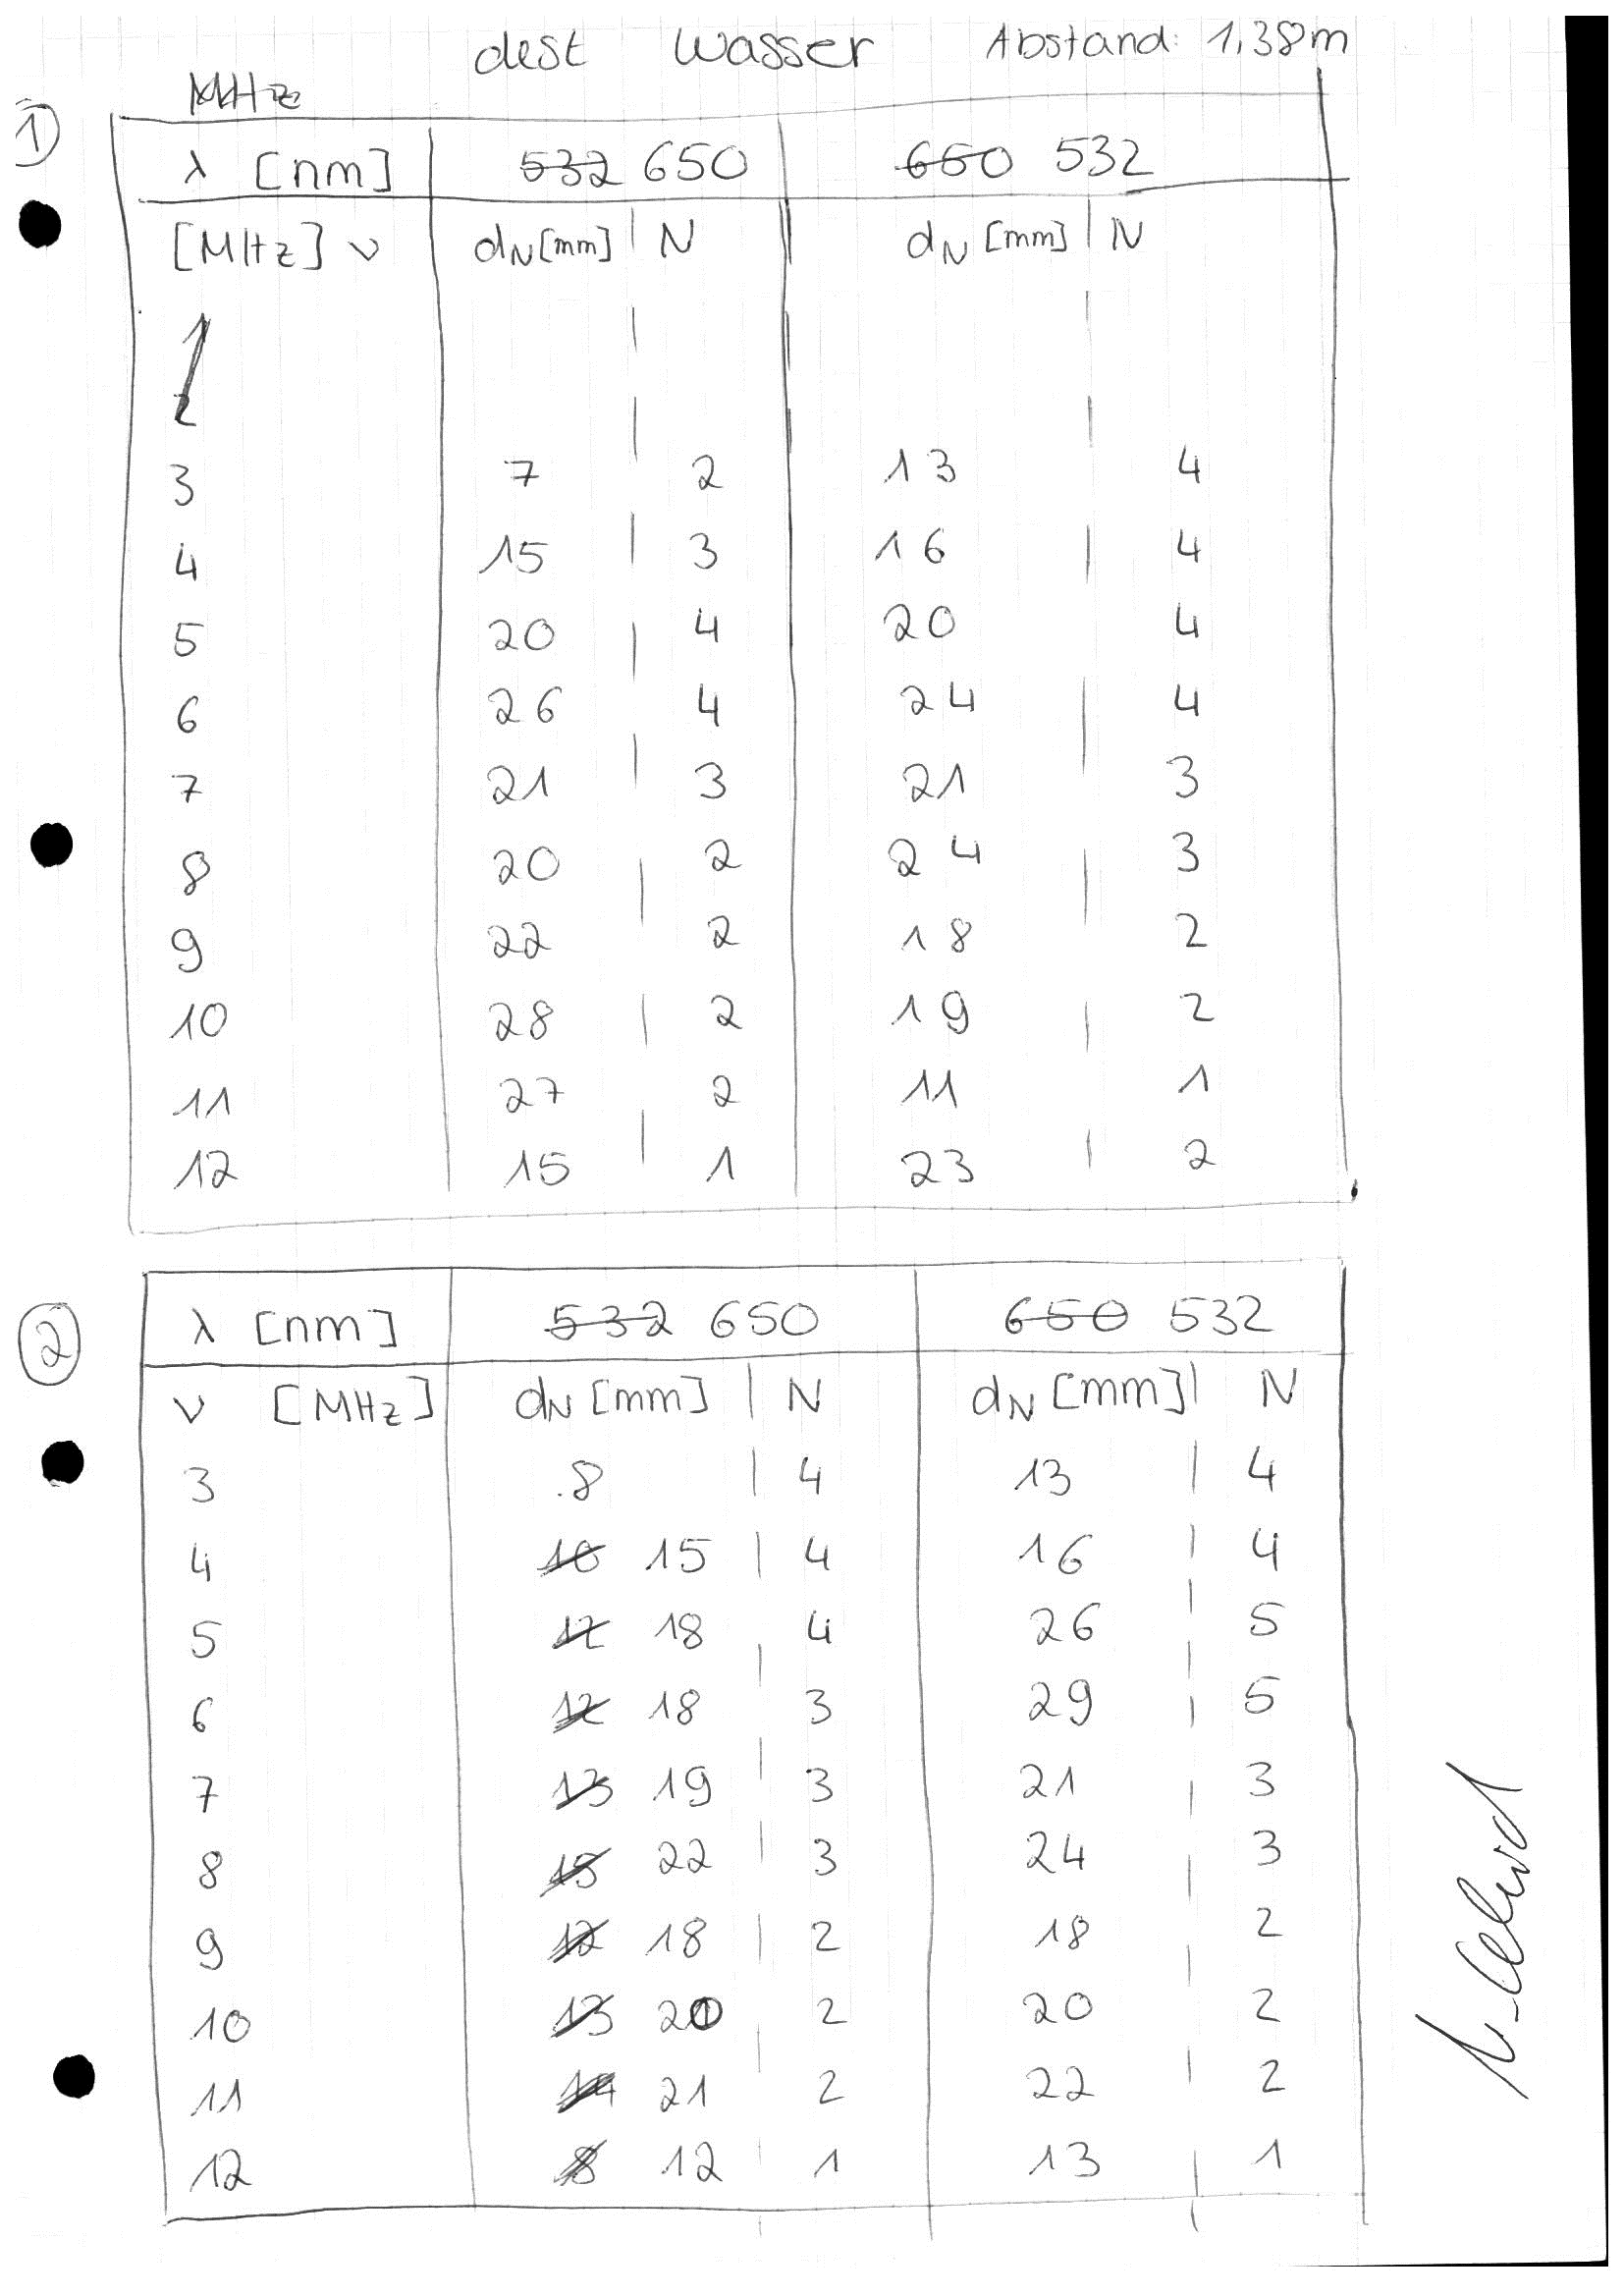
\includegraphics[scale=0.8]{Graphik/S12b}
\caption{Versuchsaufbau$^{\cite{A}}$}
\end{figure}
\newpage

\begin{figure}[h]
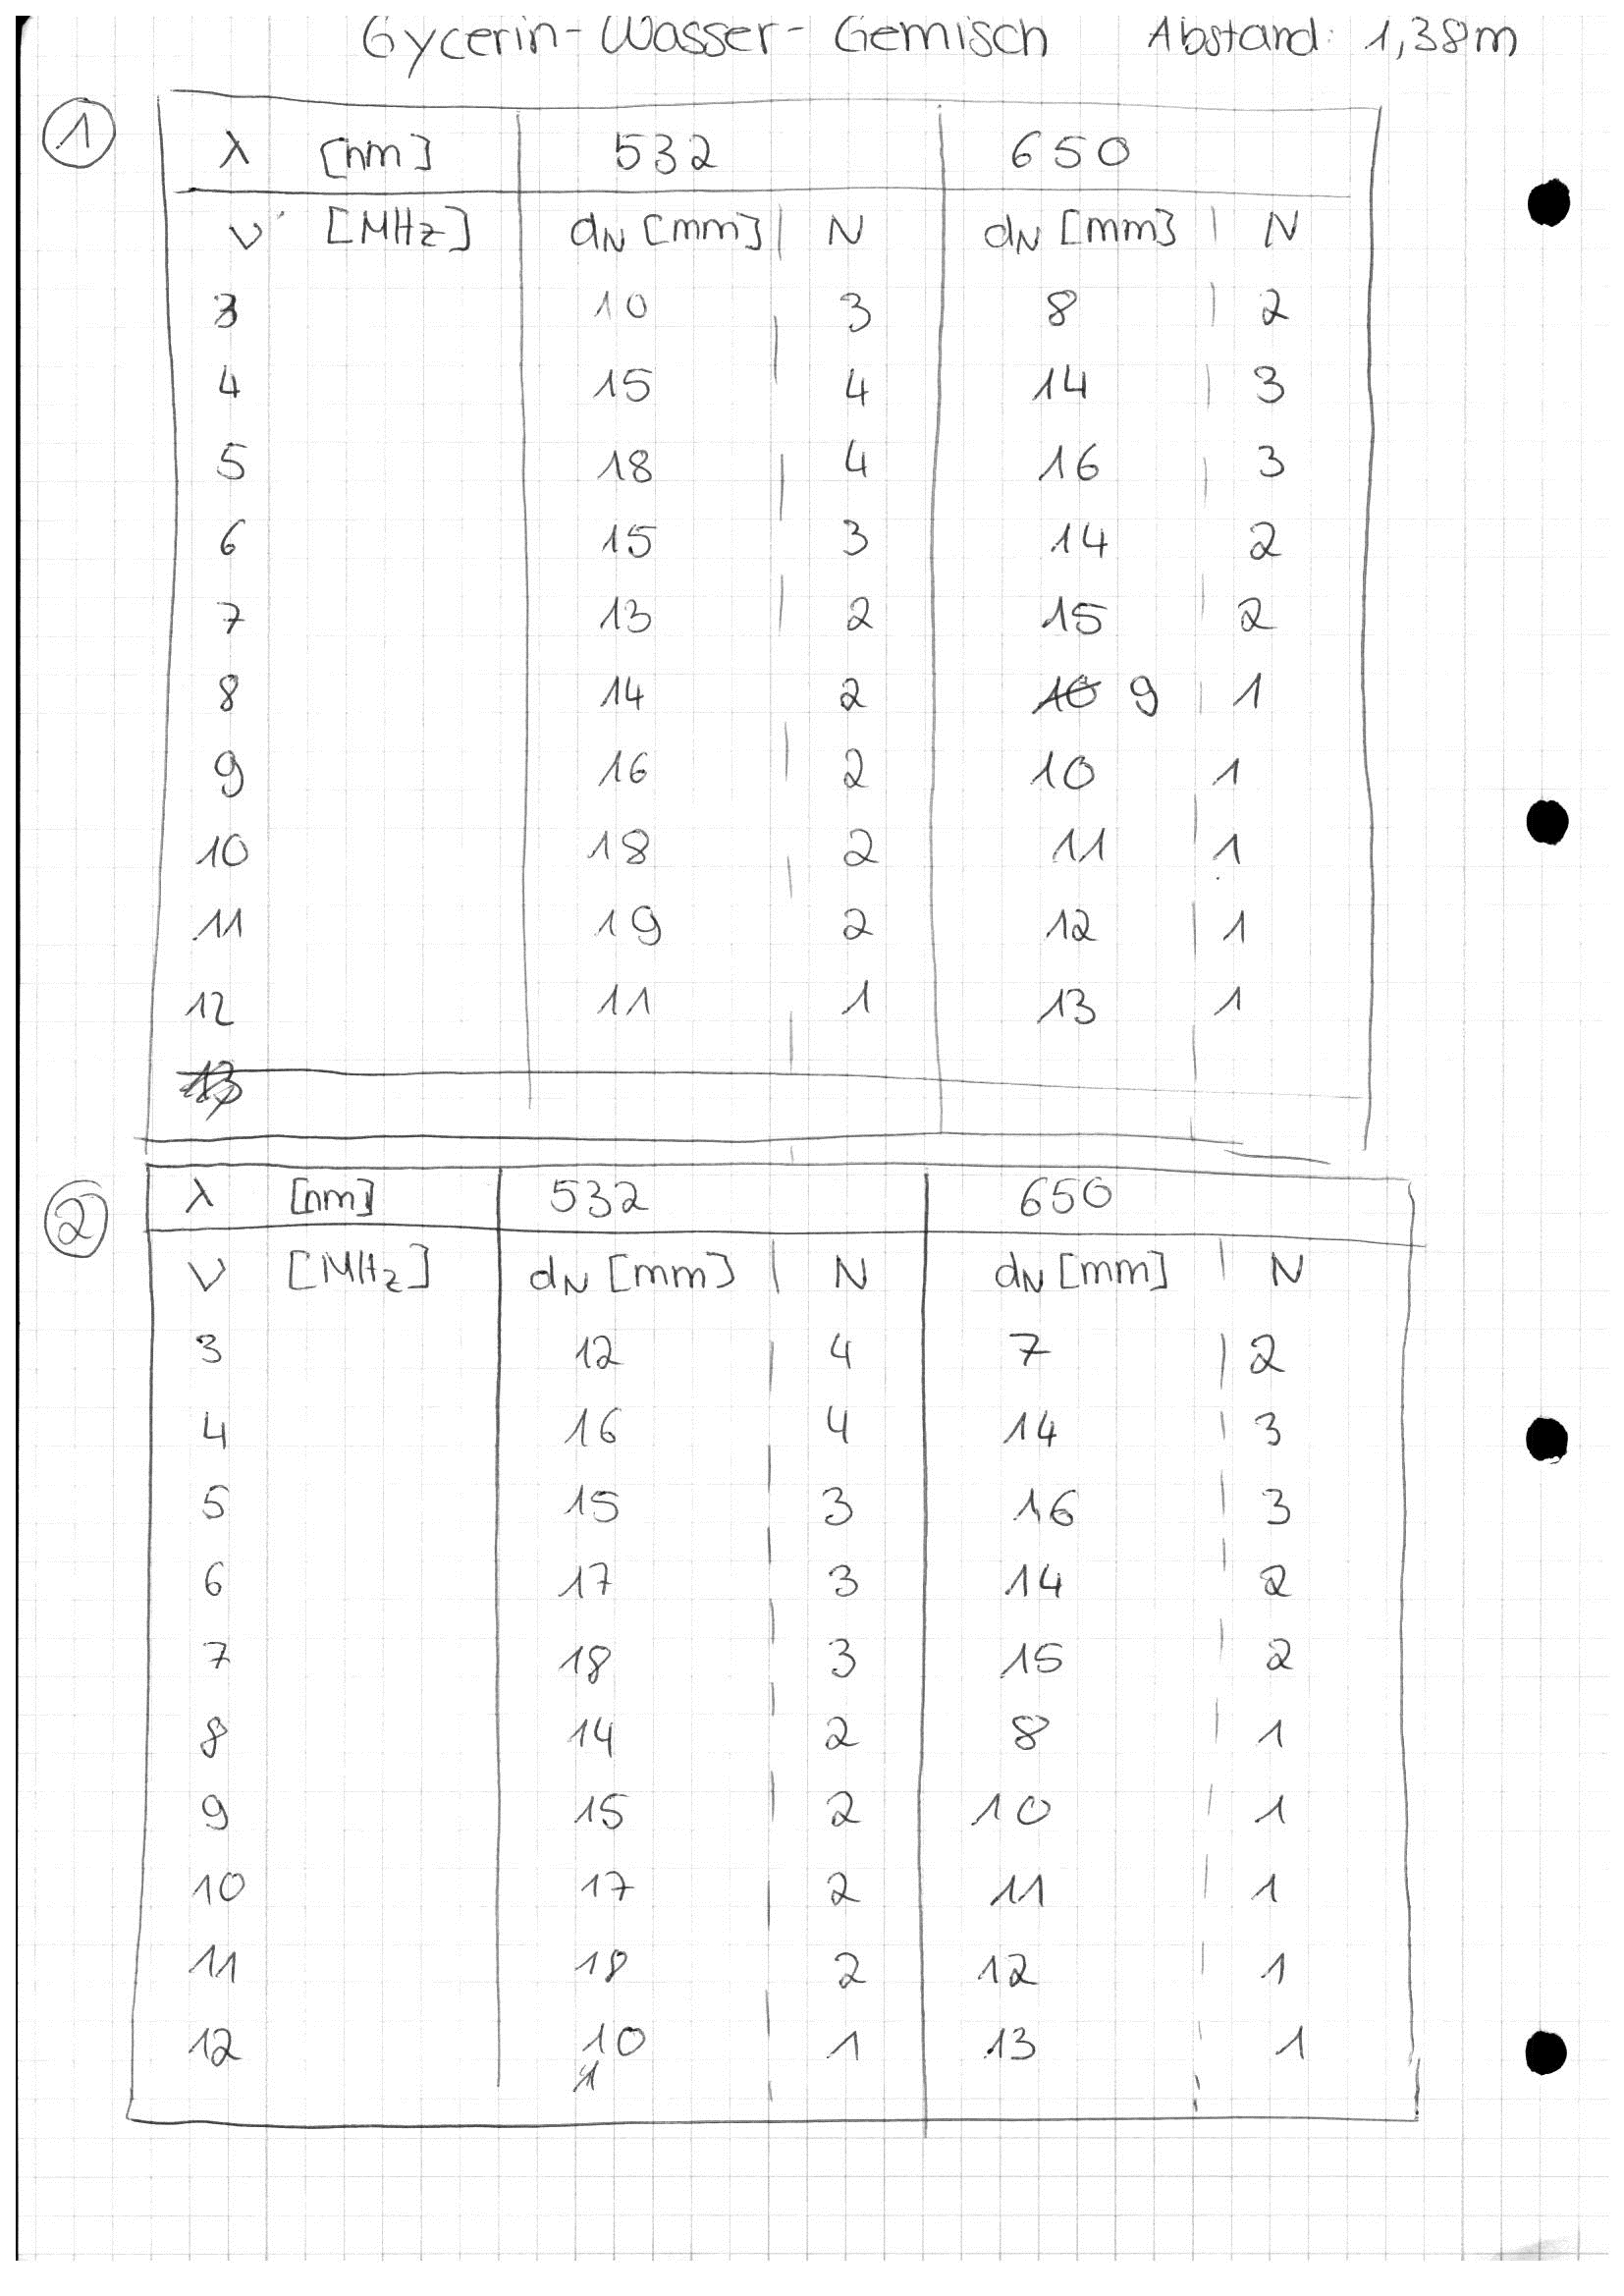
\includegraphics[scale=0.8]{Graphik/S12b2}
\caption{Versuchsaufbau$^{\cite{A}}$}
\end{figure}
\end{document}